\documentclass[aspectratio=169]{beamer}
\usetheme{Madrid}
\usecolortheme{beaver}

\usepackage[T1]{fontenc}
\usepackage[utf8]{inputenc}
\usepackage{amsmath}
\usepackage{siunitx}
\usepackage{booktabs}

\title[Vector-Like Top Partner Search]{Single Production of a Vector-Like Top Partner\\via the Recoil-Mass Technique}
\author[Valle \textit{et al.}]{Higinio Valle \and Cristina Oropeza \and Oscar Ochoa}
\institute[UIA]{Universidad Iberoamericana, CDMX, México}
\date{\today}

\begin{document}

\begin{frame}
  \titlepage
\end{frame}

\begin{frame}{Overview}
  \begin{itemize}
    \item Motivation for vector-like top partners and the recoil-mass strategy
    \item Benchmark model, simulated samples, and analysis workflow
    \item Event-selection highlights and baseline performance
    \item Impact of ISR and beam polarization on sensitivity
    \item Discovery reach in the $(m_{T},\kappa)$ plane and outlook
  \end{itemize}
\end{frame}

\begin{frame}{Motivation}
  \begin{itemize}
    \item Vector-like quarks help stabilize the Higgs potential and appear in composite/little Higgs scenarios.
    \item A clean $e^{+}e^{-}$ environment allows precise studies of single-production channels.
    \item Recoil-mass techniques provide mass-agnostic and decay-mode-agnostic searches that remain sensitive across wide $m_{T}$ ranges.
    \item Objective: quantify discovery potential for single-$T$ production at $\sqrt{s}=\SI{3}{TeV}$ with \SI{5}{ab^{-1}}.
  \end{itemize}
\end{frame}

\begin{frame}{Model and Benchmarks}
  \begin{columns}[T]
    \column{0.58\textwidth}
      \begin{itemize}
        \item Signal: $e^{+}e^{-}\rightarrow T\,\bar{t}$ with effective coupling $\kappa$ at the $T$--top--gauge vertex.
        \item Benchmark masses: $m_{T}=\{1.2,1.6,2.0,2.4\}\,\si{TeV}$ with widths from dedicated simulations.
        \item Reference coupling: $\kappa=0.20 \Rightarrow \Gamma_{T}\approx\SI{22.3}{GeV}$ for $m_{T}=\SI{1.2}{TeV}$.
        \item Additional samples scan $\kappa\in\{0.10,\dots,0.60\}$ to map the discovery reach.
      \end{itemize}
    \column{0.38\textwidth}
      \centering
      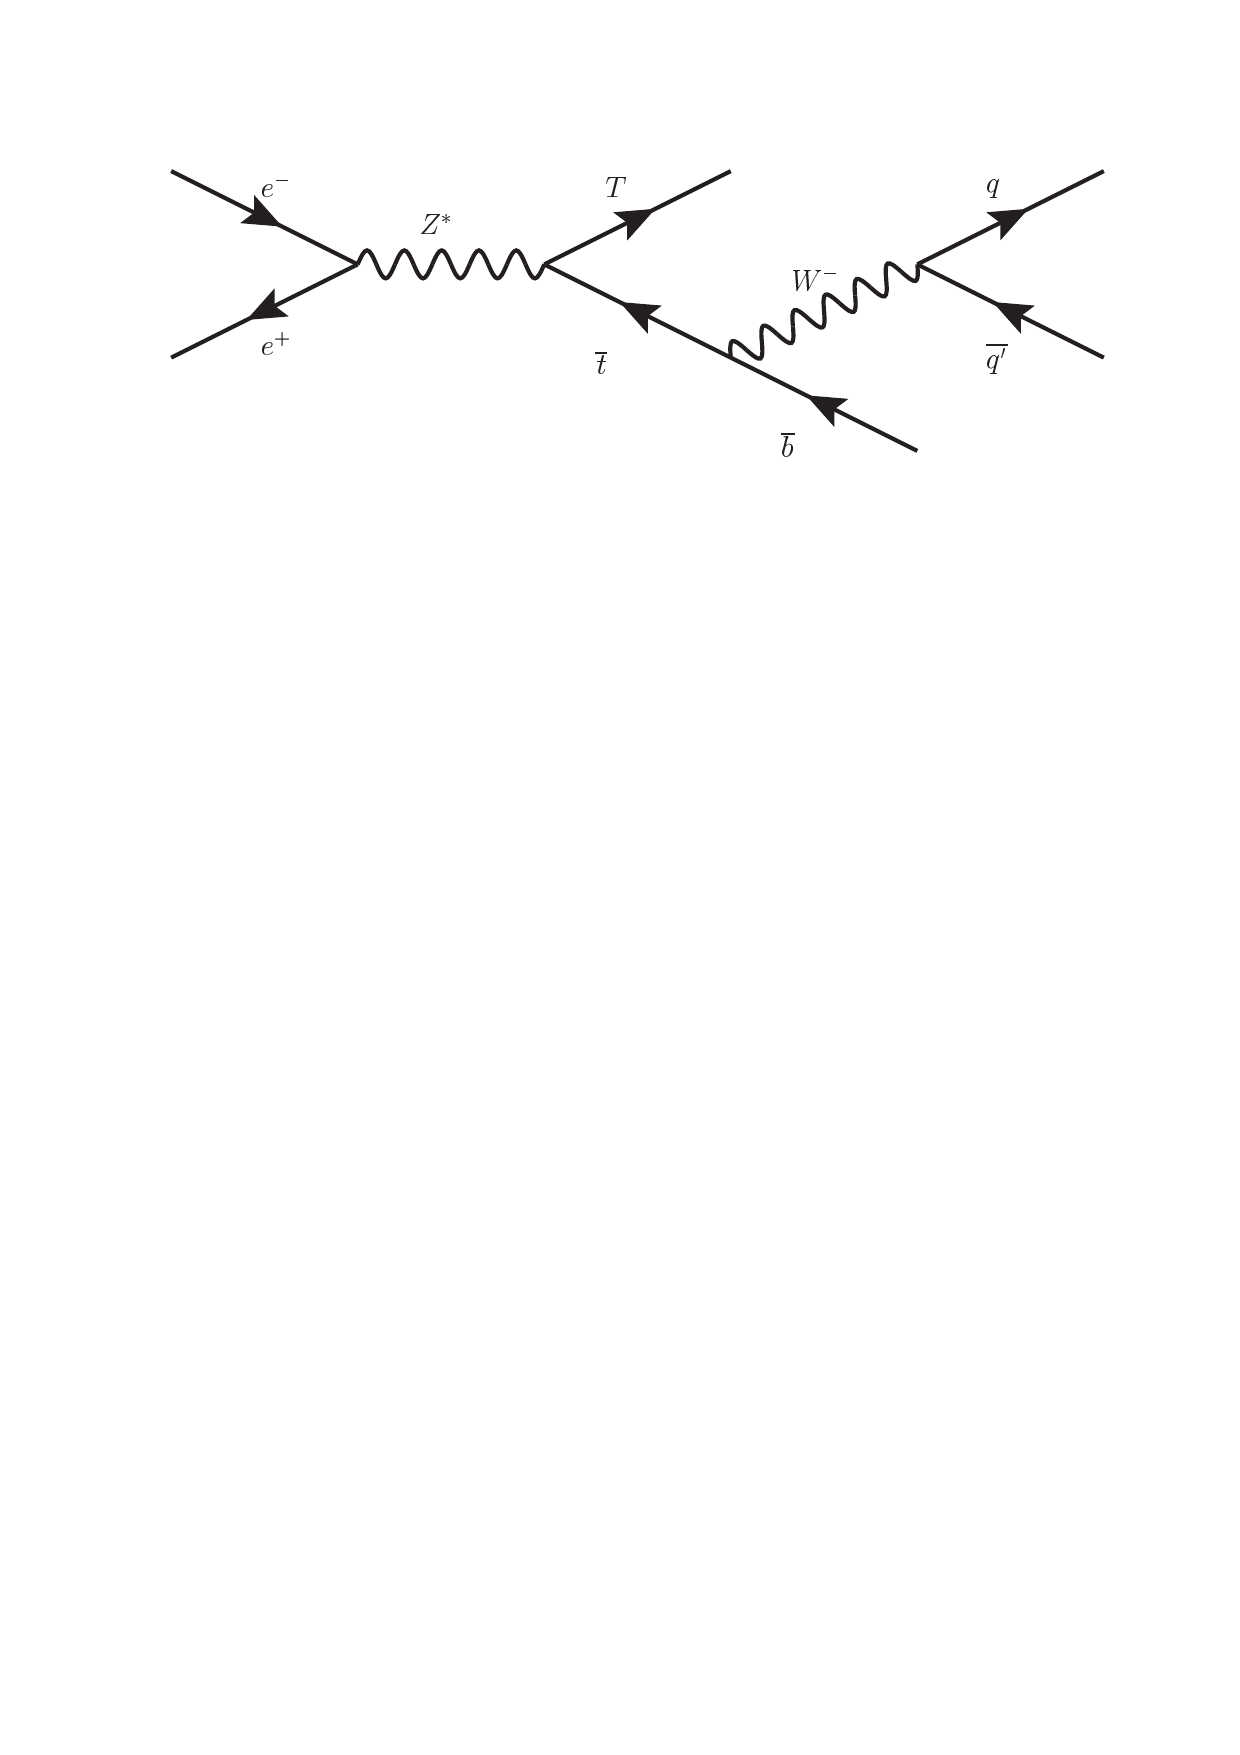
\includegraphics[width=\linewidth]{figs/feynman_diagram.png}
  \end{columns}
\end{frame}

\begin{frame}{Event Samples and Reconstruction}
  \small
  \[
    \mathcal{L}_{\text{eff}} \supset \kappa_{T} \left\{
      \sqrt{\tfrac{\zeta_{Tq}^{W}}{\Gamma_{W}}} \tfrac{g}{\sqrt{2}}
        \big[\bar{T}_{L/R} W^{+}_{\mu} \gamma^{\mu} d_{L/R}\big]
      + \sqrt{\tfrac{\zeta_{Tt}^{Z}}{\Gamma_{Z}}} \tfrac{g}{2 c_{W}}
        \big[\bar{T}_{L/R} Z_{\mu} \gamma^{\mu} u_{L/R}\big]
      - \sqrt{\tfrac{\zeta_{Tt}^{H}}{\Gamma_{H}}} \tfrac{M}{v}
        \big[\bar{T}_{R/L} H u_{L/R}\big]
    \right\} + \text{h.c.}
  \]
  \begin{itemize}
    \item Model: Mathieu Buchkremer et al. “Model-independent framework for searches of top partners”(Nuclear Physics
B 876.2 (2013), págs. 376-417.).
    \item Generation: \textsc{MadGraph5\_aMC@NLO} + \textsc{MadSpin} with \textsc{Pythia}~8 showering.
    \item Backgrounds: $t\bar{t}$, $t\bar{t}Z$, $t\bar{t}h$, $W^{+}W^{-}Z$, normalized to \SI{5}{ab^{-1}}.
    \item Two configurations: baseline (no ISR, unpolarized) and ISR + $P_{e^{-}}=+80\%$.
  \end{itemize}
\end{frame}

\begin{frame}{Selection Strategy}
  \begin{columns}[T]
    \column{0.54\textwidth}
      \begin{itemize}
        \item Identify a high-$p_{T}$ Cambridge--Aachen $R=1.0$ fat jet tagged with the Johns Hopkins top-tagger.
        \item Require at least one $b$-tagged subjet/small-$R$ jet to suppress light-flavor backgrounds.
        \item Constrain event kinematics: $E_{\text{miss}}<\SI{1}{TeV}$ and $m_{\text{recoil}}>\SI{1.1}{TeV}$.
      \end{itemize}
    \column{0.42\textwidth}
      \centering
      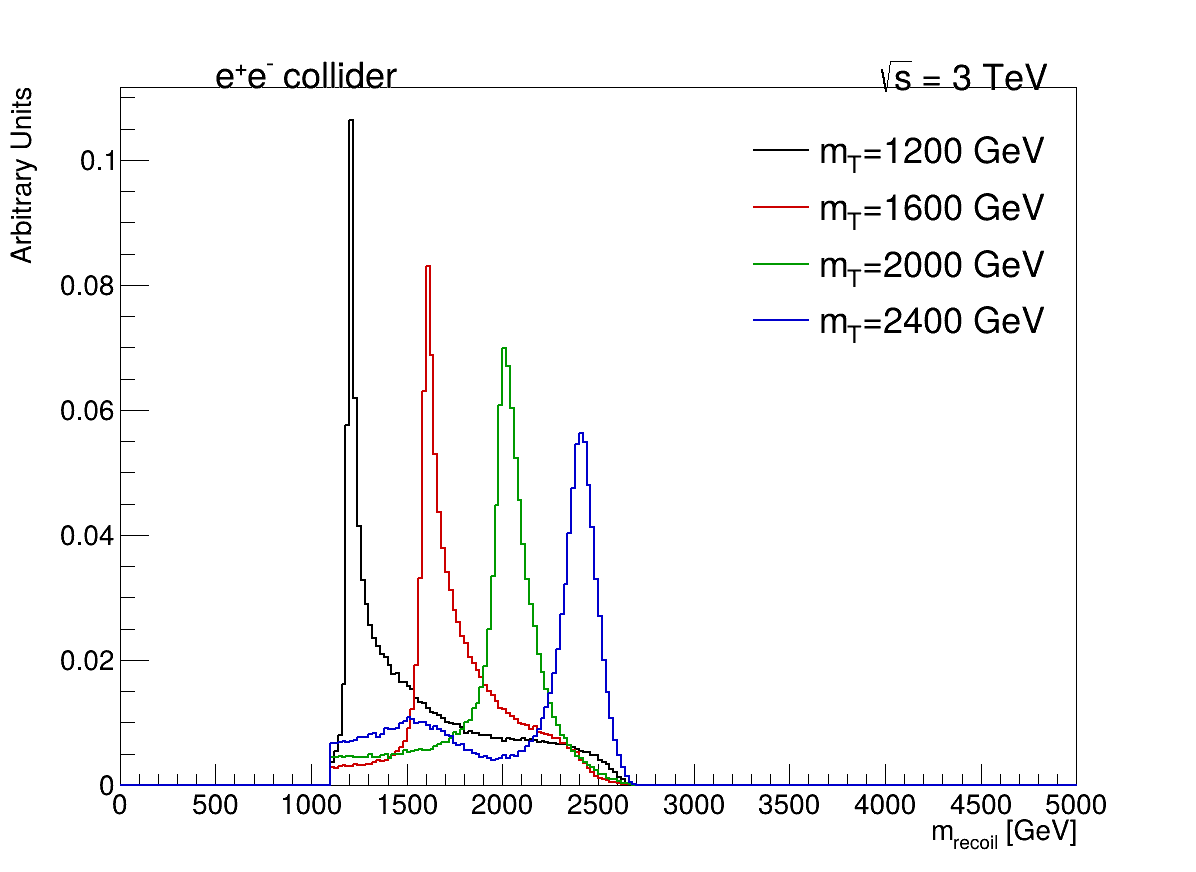
\includegraphics[width=\linewidth]{figs/signals_after_cuts.png}
  \end{columns}
\end{frame}

\begin{frame}{Baseline Performance}
  \begin{itemize}
    \item $t\bar{t}$ reduced from $\mathcal{O}(10^{5})$ to $2.3\times 10^{3}$ events after the full selection.
    \item Signal efficiency for $m_{T}=\SI{1.2}{TeV}$ retains $\sim16\%$ of events ($\approx$199 / 1232) at $L=\SI{5}{ab^{-1}}$.
    \item Total background after full selection: $B\approx\num{6940}$ events for $L=\SI{5}{ab^{-1}}$.
    \item Counting significance for $\kappa=0.20$: $Z=2.35$ at $m_{T}=\SI{1.2}{TeV}$ for $L=\SI{5}{ab^{-1}}$.
  \end{itemize}
\end{frame}

\begin{frame}{Significance Summary}
  \begin{columns}[T]
    \column{0.46\textwidth}
      \small
      \begin{tabular}{c S[table-format=1.2] S[table-format=1.2]}
    \toprule
    $m_{T}$ [TeV] & {$Z_{\text{base}}$} & {$Z_{\text{ISR+pol}}$} \\
    \midrule
    1.2 & 2.35 & 1.72 \\
        1.6 & 1.97 & 1.31 \\
        2.0 & 1.15 & 0.67 \\
        2.4 & 0.30 & 0.15 \\
        \bottomrule
      \end{tabular}
    \column{0.48\textwidth}
      \centering
      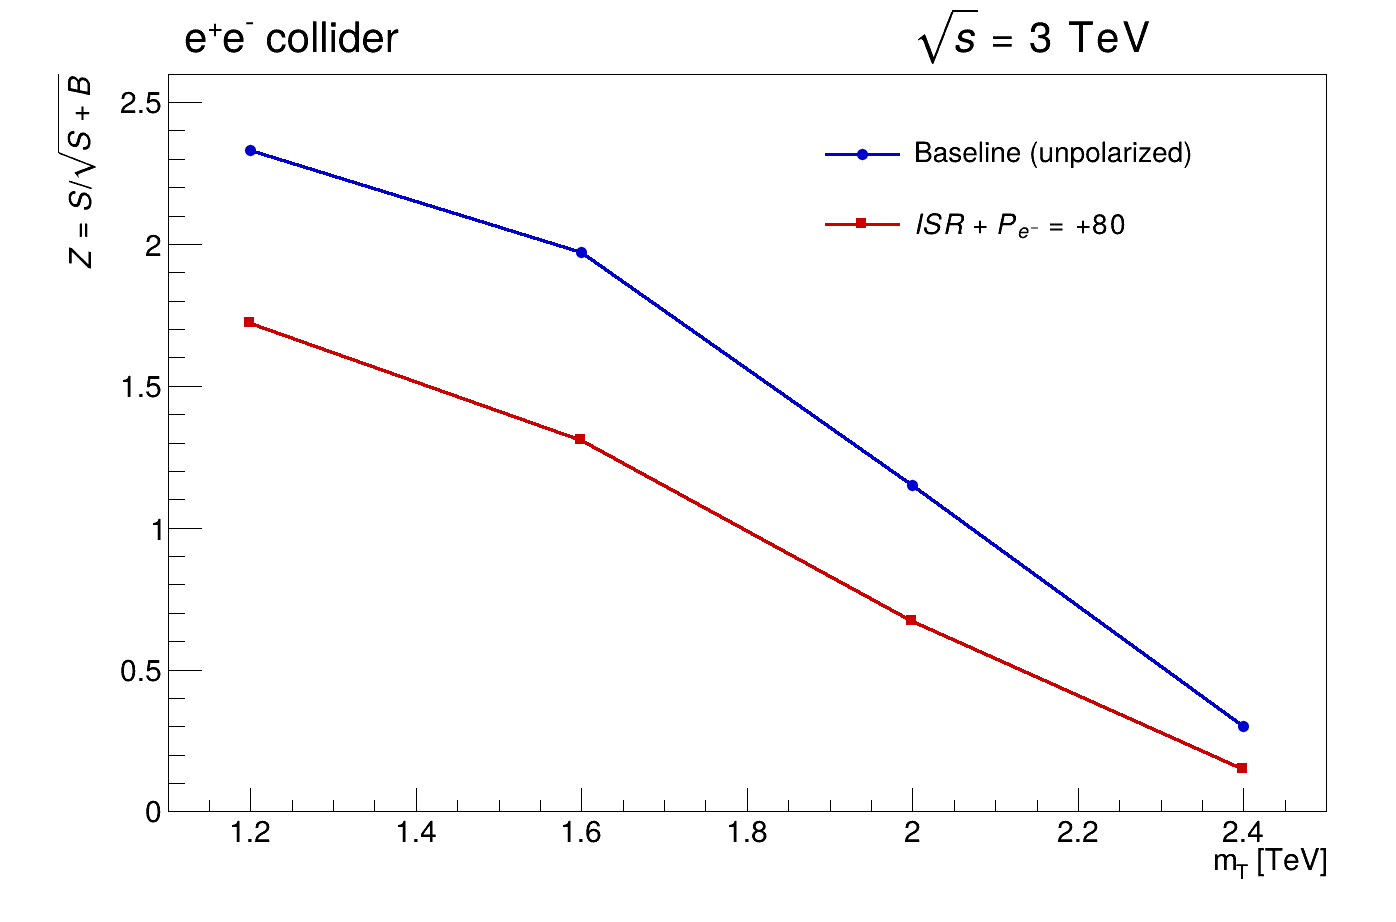
\includegraphics[width=\linewidth]{figs/significance_vs_mass.png}
  \end{columns}
\end{frame}

\begin{frame}{Recoil-Mass Spectrum}
  \centering
  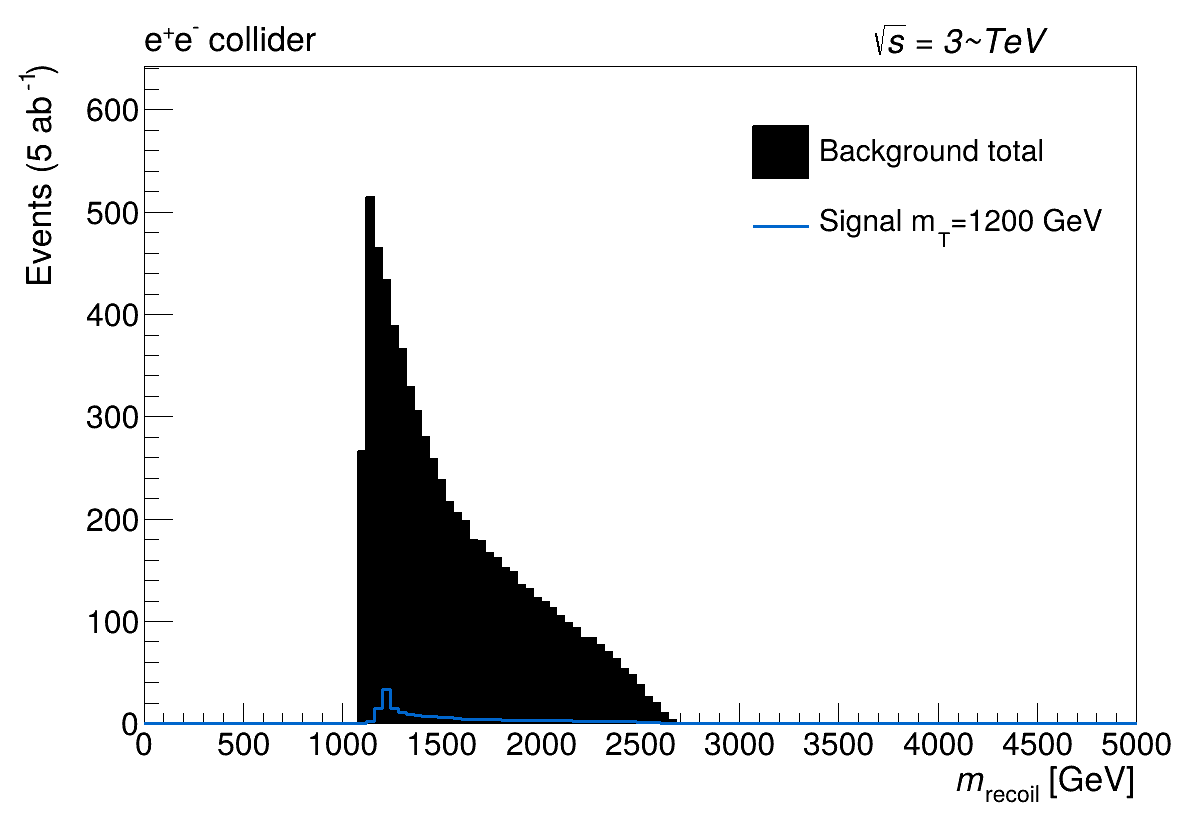
\includegraphics[height=0.72\textheight]{figs/recoil_baseline.png}
\end{frame}

\begin{frame}{Impact of ISR and Polarization}
  \begin{columns}[T]
    \column{0.48\textwidth}
    \begin{itemize}
      \item ISR increases background acceptance to $B=\num{9789}$.
      \item Signal yield drops from 199 to 172 events at $m_{T}=\SI{1.2}{TeV}$.
      \item Net effect: $\sim25\%$ loss in counting significance.
    \end{itemize}
    \column{0.5\textwidth}
    \centering
    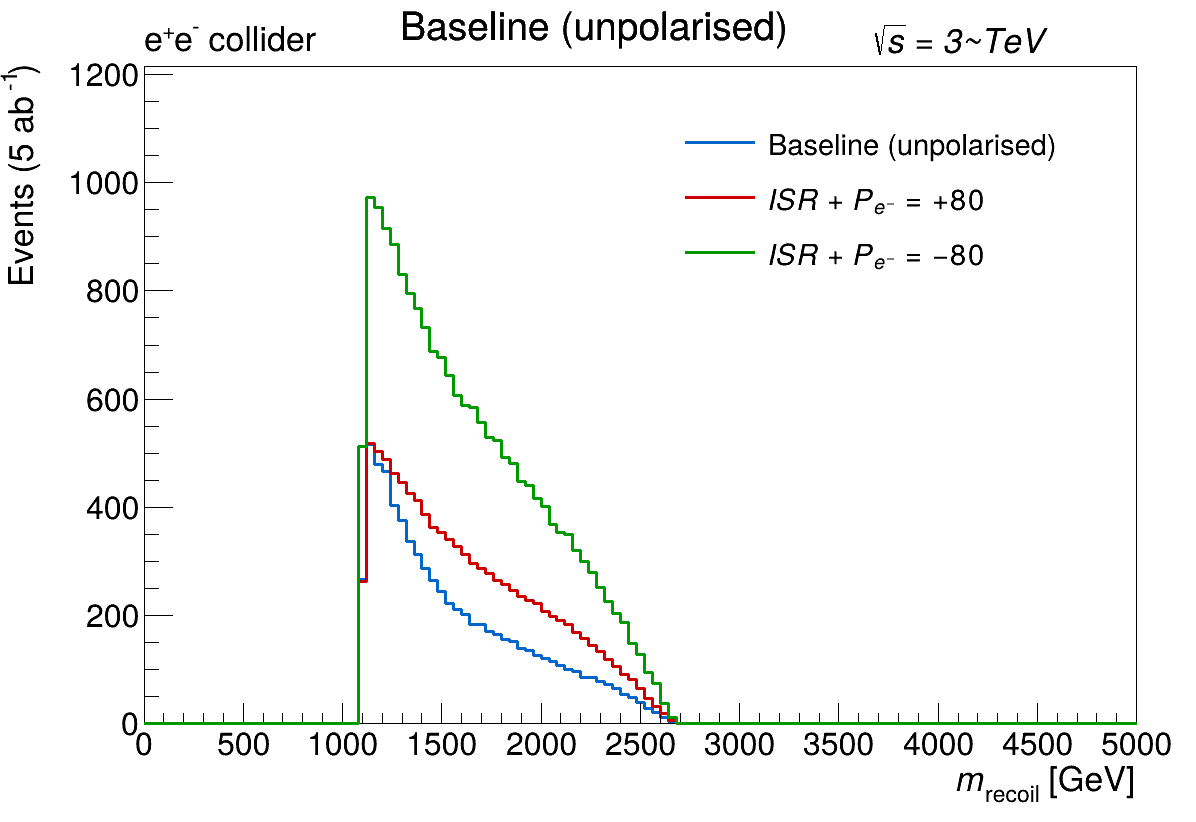
\includegraphics[height=0.55\textheight]{figs/recoil_comparison.png}
  \end{columns}
\end{frame}

\begin{frame}{Coupling Scan}
  \begin{columns}[T]
    \column{0.48\textwidth}
      \begin{itemize}
        \item Dedicated samples map $Z=S/\sqrt{S+B}$ versus $(m_{T},\kappa)$.
        \item Baseline (no ISR) reaches $Z\approx5$ at $(1.2\,\si{TeV},\,\kappa=0.30)$.
        \item ISR + $P_{e^{-}}=+80\%$ shifts the reach to $Z\approx3.7$ at the same point.
        \item Sensitivity falls below $Z=1$ near $m_{T}\gtrsim\SI{2}{TeV}$ unless $\kappa\gtrsim 0.4$.
      \end{itemize}
    \column{0.24\textwidth}
      \centering
      
\includegraphics[width=\linewidth]{figs/kappa_scan_baseline.png}\\[-0.5ex]
      {\scriptsize Baseline}
    \column{0.24\textwidth}
      \centering
      
\includegraphics[width=\linewidth]{figs/kappa_scan_plus80ISR.png}\\[-0.5ex]
      {\scriptsize ISR + $P_{e^{-}}=+80\%$}
  \end{columns}
\end{frame}

\begin{frame}{Summary and Outlook}
  \begin{block}{Summary}
    Baseline selection reaches about 2.35 sigma at 1.2 TeV with kappa 0.20, retaining roughly 16 percent of the signal while remaining mass and decay-mode agnostic across the scanned benchmarks.\\
    ISR with plus-eighty-percent electron polarisation reduces the yield but the recoil observable keeps broad sensitivity over the mass versus kappa plane.
  \end{block}
  \begin{block}{Next Steps}
    Optimise the selection separately for low and high masses, extend the dedicated studies to additional kappa benchmarks, and incorporate ISR-aware observables to recover significance.
  \end{block}
\end{frame}

\begin{frame}{Backup: Baseline Cutflow}
  \small
  \centering
  \begin{tabular}{l S[table-format=5.1] S[table-format=6.1]}
    \toprule
    Selection step & {Signal} & {$t\bar{t}$} \\
    \midrule
    All events & 1232.3 & 95706.0 \\
    Fat-jet preselection & 1232.0 & 95335.1 \\
    Top tagged & 401.4 & 41535.0 \\
    Substructure tag & 348.6 & 37869.4 \\
    Isolation veto & 215.1 & 31975.5 \\
    $m_{\text{recoil}}>\SI{1.1}{TeV}$ & 206.1 & 5897.1 \\
    $E_{\text{miss}}<\SI{1}{TeV}$ & 198.6 & 5654.6 \\
    BDT$_{t\bar{t}}$ & 189.2 & 4244.3 \\
    BDT$_{1200}$ & 187.3 & 4122.1 \\
    Final (BDT$_{2400}$) & 110.0 & 2322.6 \\
    \bottomrule
  \end{tabular}
\end{frame}

\end{document}
